\documentclass{article}
\usepackage[utf8]{inputenc}
\usepackage[spanish]{babel}
\usepackage{listings}
\usepackage{graphicx}
\graphicspath{ {images/} }
\usepackage{cite}

\begin{document}

\begin{titlepage}
    \begin{center}
        \vspace*{1cm}
            
        \Huge
        \textbf{PROCESAMIENTO DE IMÁGENES  }
            
        \vspace{0.5cm}
        \LARGE
        Parcial 2
            
        \vspace{1.5cm}
            
        \textbf{Sergio Alberto Giraldo  Salazar \\ Diego Fernando Urbano Palma }
        
        \vfill
            
        \vspace{0.8cm}
            
        \Large
        Departamento de Ingeniería Electrónica y Telecomunicaciones\\
        Universidad de Antioquia\\
        Medellín\\
        Septiembre de 2021
            
    \end{center}
\end{titlepage}

\tableofcontents
\newpage
\section{Análisis del problema}\label{intro}
En el presente parcial se nos pide dar una interpretación de una imagen donde se submuestrea o se sobremuestrea para que sea compatible con la matriz de leds que se va montar en TINKERCAD.
Con el presente proyecto se evidencian  las siguientes dificultades, como lo serian la interpretación de datos por parte del TINKERCAD.\\
Otra dificultad para el proyecto es entender las matrices de datos que nos van a mostrar en el camino, como lo es la matriz RGB la cual nos dan el color de cada pixel para poder generar un código que nos  submuestre o sobremuestre la imagen. \\Saber que es sobremuestreo  y submuestre ya que es el eje de la practica 2 que en este momento estamos presentando. \\
Manejar correctamente las librerías de Arduino para darle el color deseado a nuestros leds mostrando la imagen después de haber completado el los procesos para tratar una imagen.


\section{funcionamiento del circuito} \label{contenido}

\begin{figure}[h]
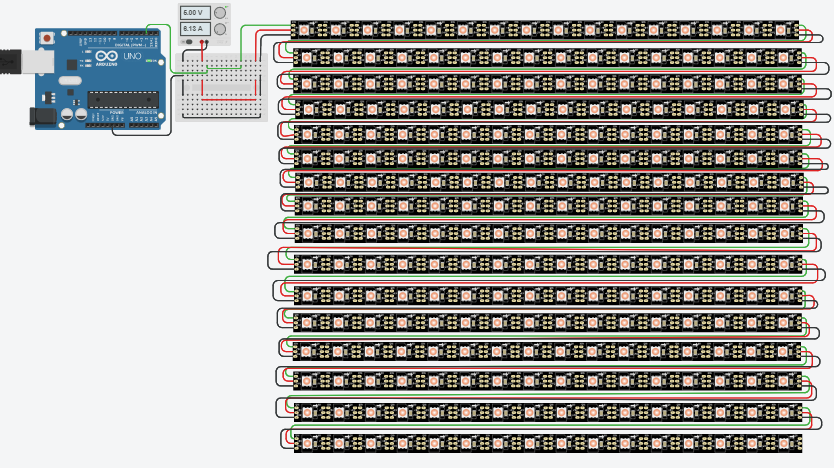
\includegraphics[width=10cm]{Simulación.png}
\centering
\caption{Matriz de leds}
\label{fig:matriz de leds}
\end{figure}
\label{contenio}
En la imagen se plantea una matriz de leds 16*16 donde el primer led a tomar en cuenta será el superior a la izquierda y de allí se ira avanzando hacia la derecha, decidimos tomar este orden para tener una mayor facilidad de compresión de como se ira reflejando los cambios en cada led.



\section{Plantiamiento de soluciones }

\subsection{Información de la imagen  }

Para poder manejar la información de la imagen en el tinkercard lo que tenemos que hacer es por medio de C++ transformar los datos de cada pixel en una matriz, modificarla y pegar dicha matriz como constantes en el simulador para que de esta manera podamos manejar la información de cada uno de los pixeles, como se muestra en el pseudo código \ref{codigo_ejemplo}. 
\begin{lstlisting}[language=C++, label=codigo_ejemplo]

// Incluimos las librerias necesarias para leer
//la imagen y podemos realizar nuestro codigo
#include <iostream>
#include "QImage"
#include "string.h"
#include "fstream"
using namespace std;

int main()
{
    ///////// LECTURA DE PIXELES DE LA IMAGEN //////////
//declaramos las clases para la lectura de imagen
// y la de manipulacion de archivos de texto
    QImage imagen("direccion de la imagen ");
    fstream matriz("nombre del archivo de texto", fstream::app);
    unsigned InfLeds[3][16][16], azul,verde,rojo;
    string cadena;
// se hace una cadena de for para que se se obtenga
//la informacion de cada una de los pixeles de la imagen

    for(iterador <= altura de la imagen)
    {
        for(iterador<= ancho de la imagen)
        {

           InfLeds[0][iterador altura][iterador ancho]=azul;
           InfLeds[1][iterador altura][iterador ancho]=verde;
           InfLeds[2][iterador altura][iterador ancho]=rojo;
        }
    }


 /////////////////////////////////////////////////////////////////////////////////////////

    /// ingresar datos al txt ///
    for(iterador <= altura de la matriz de leds)
    {   cadena=cadena+"[";
        for(iterador<= ancho de la matriz de leds)
        {

           cadena=cadena+"azul,rojo,verde";
           matriz<<cadena;

        }
         cadena=cadena+"]";
    }



    return 0;
}
\end{lstlisting}
En la sección \ref{imagenes}, se presentará como añadir ilustraciones al texto.

\section{Inclusión de imágenes} \label{imagenes}




Las secciones (\ref{intro}), (\ref{contenido}) y (\ref{imagenes}) dependen del estilo del documento.

\bibliographystyle{IEEEtran}
\bibliography{references}

\end{document}
